
\section{Student's t-distribution ($t_\nu$)}

\begin{table}[H]
    \hfill
    \begin{minipage}{0.45\linewidth}
        \begin{figure}[H]
            \centering
            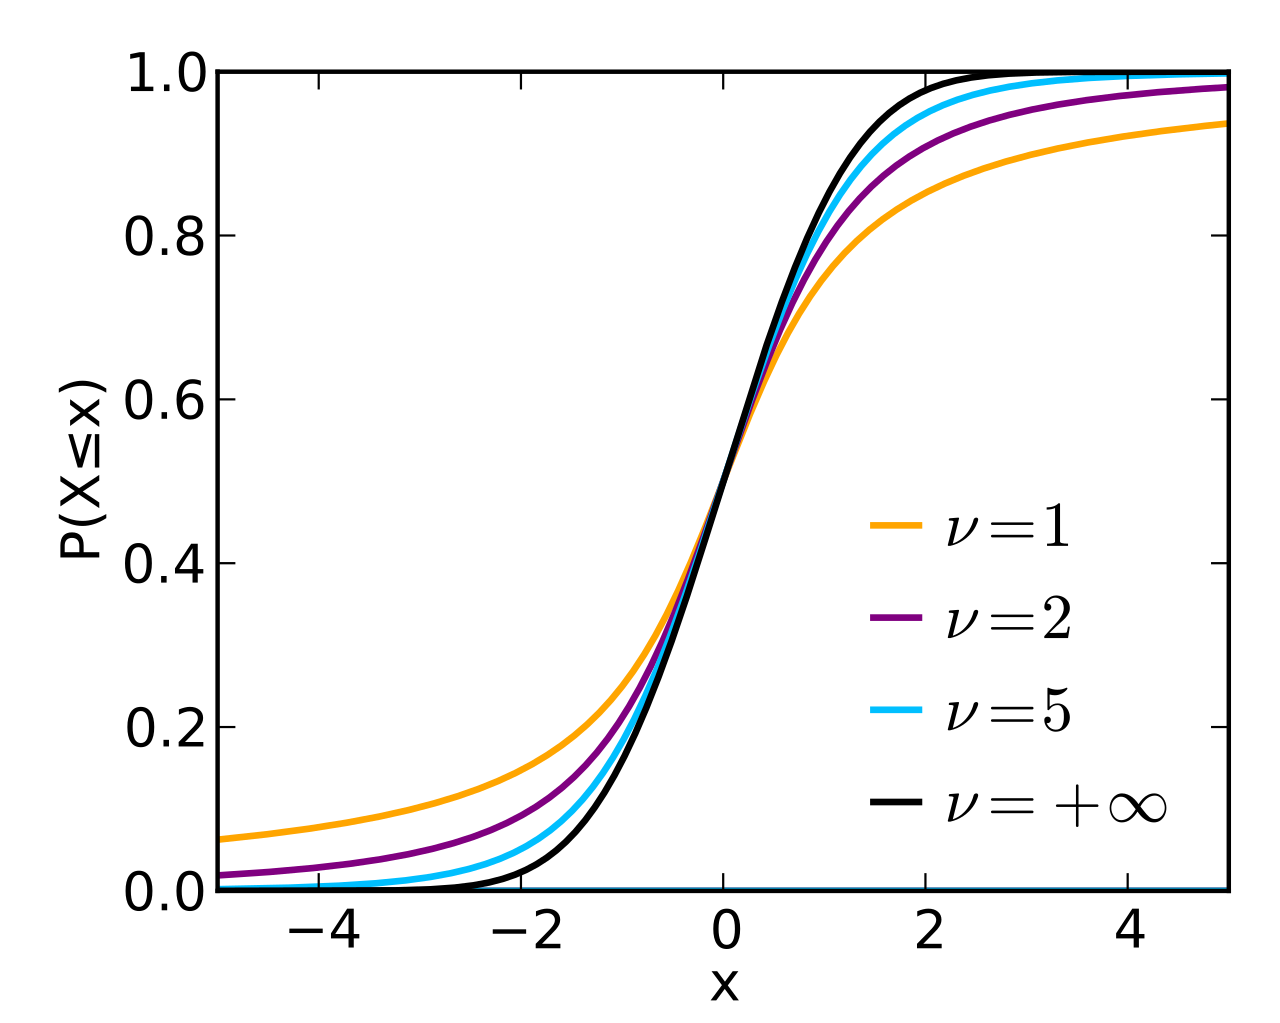
\includegraphics[
                width=\linewidth,
                height=5cm,
                keepaspectratio,
            ]{images/distributions/Student_t_cdf.svg.png}
            \caption{Student's t-distribution: PDF \cite{wiki/Students_t-distribution}}
        \end{figure}
    \end{minipage}
    \hfill
    \begin{minipage}{0.45\linewidth}
        \begin{figure}[H]
            \centering
            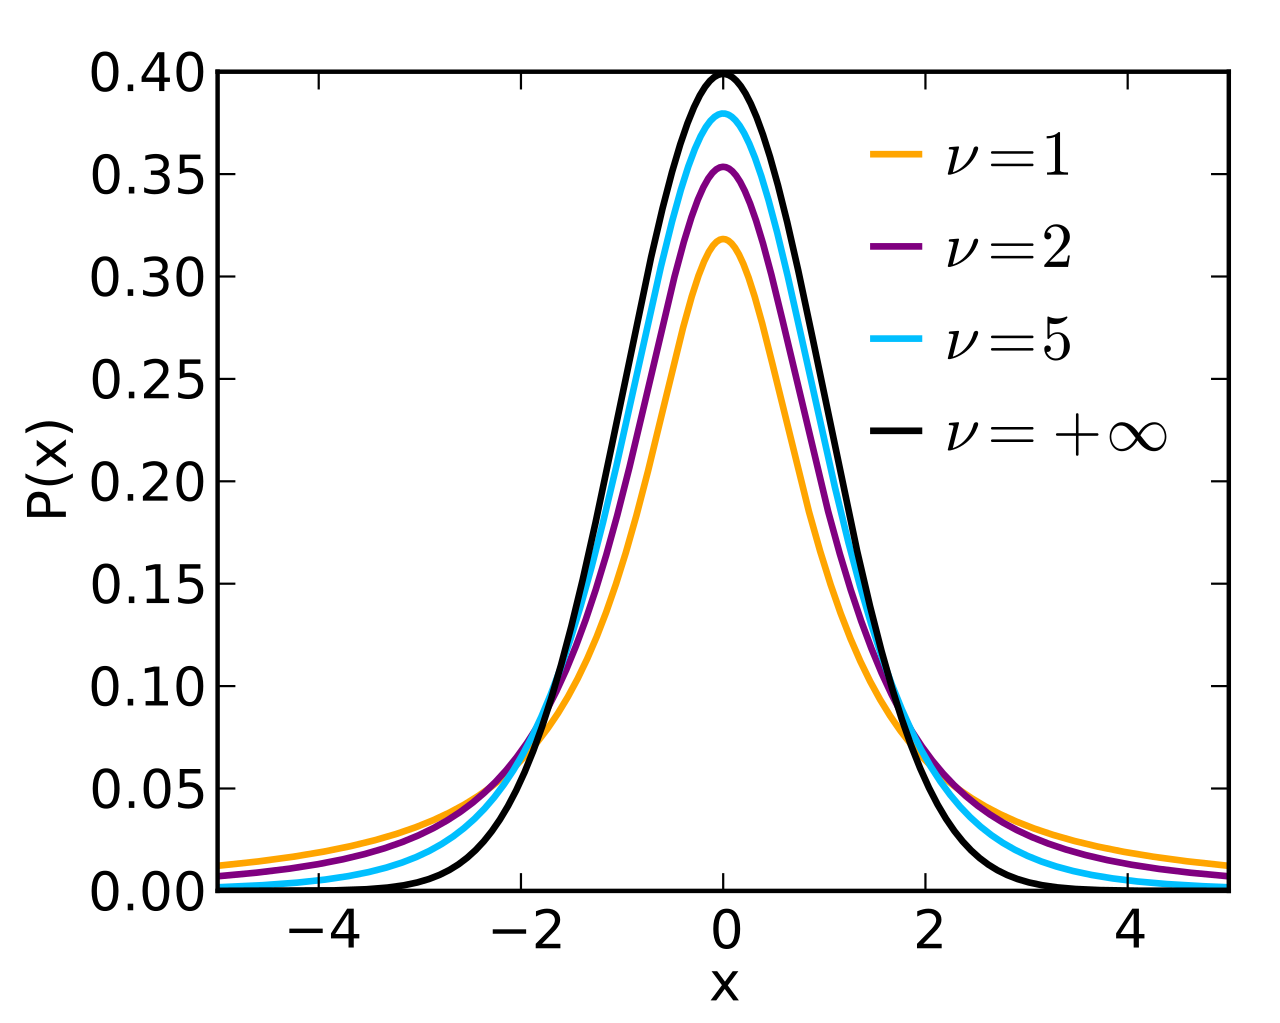
\includegraphics[
                width=\linewidth,
                height=5cm,
                keepaspectratio,
            ]{images/distributions/Student_t_pdf.svg.png}
            \caption{Student's t-distribution: CDF \cite{wiki/Students_t-distribution}}
        \end{figure}
    \end{minipage}
    \hfill
\end{table}



\begin{enumerate}
    \item Student’s t-density is symmetric around zero.
    The symmetry implies the following relation for the $p$-th quantile: $x _p ( f _t ) = -x_{1- p} ( f _t )$.
    \hfill \cite{statistics/book/Statistics-for-Data-Scientists/Maurits-Kaptein}

    \item The skewness is zero only when the degrees of freedom are larger than $3$.
    To have a finite kurtosis the degrees of freedom should be larger than $4$.
    \hfill \cite{statistics/book/Statistics-for-Data-Scientists/Maurits-Kaptein}
\end{enumerate}




\subsection{Summary}

\begin{enumerate}
    \item \textbf{Parameters}: ${\displaystyle \nu >0}$ degrees of freedom (real, almost always a positive integer)
    \hfill \cite{wiki/Students_t-distribution}

    \item \textbf{Support}: $  {\displaystyle x\in (-\infty ,\infty )} $
    \hfill \cite{wiki/Students_t-distribution}

    \item \textbf{PDF}: $  {\displaystyle {\dfrac {\Gamma {\left({\dfrac {\nu +1}{2}}\right)}}{{\sqrt {\pi \nu }}\,\Gamma {\left({\dfrac {\nu }{2}}\right)}}}\left(1+{\dfrac {x^{2}}{\nu }}\right)^{-{\dfrac {\nu +1}{2}}}} $
    \hfill \cite{wiki/Students_t-distribution}

    \item \textbf{CDF}:  ${\displaystyle {\dfrac {1}{2}}+x\Gamma {\left({\dfrac {\nu +1}{2}}\right)}\times {\dfrac {{}_{2}F_{1}\!\left({\dfrac {1}{2}},{\dfrac {\nu +1}{2}};{\dfrac {3}{2}};-{\dfrac {x^{2}}{\nu }}\right)}{{\sqrt {\pi \nu }}\,\Gamma {\left({\dfrac {\nu }{2}}\right)}}}}$
    where ${\displaystyle {}_{2}F_{1}}$ is the hypergeometric function
    \hfill \cite{wiki/Students_t-distribution}

    % \item \textbf{Quantile}: $  $
    % \hfill \cite{wiki/Students_t-distribution}

    \item \textbf{Mean}:  ${\displaystyle 0}$ for ${\displaystyle \nu >1,}$ otherwise undefined
    \hfill \cite{wiki/Students_t-distribution}

    \item \textbf{Median}: $ 0 $
    \hfill \cite{wiki/Students_t-distribution}

    \item \textbf{Mode}: $ 0 $
    \hfill \cite{wiki/Students_t-distribution}

    \item \textbf{Variance}:  ${\displaystyle {\dfrac {\nu }{\nu -2}}}$ for ${\displaystyle \nu >2}$, ${\displaystyle \infty }$ for ${\displaystyle 1<\nu \leq 2}$, otherwise undefined
    \hfill \cite{wiki/Students_t-distribution}

    \item \textbf{Skewness}:  ${\displaystyle 0}$ for ${\displaystyle \ \nu >3\ }$, otherwise undefined
    \hfill \cite{wiki/Students_t-distribution}

    \item \textbf{Excess kurtosis}:  ${\displaystyle {\dfrac {6}{\nu -4}}}$ for ${\displaystyle \nu >4}$, ${\displaystyle \infty }$ for ${\displaystyle 2<\nu \leq 4}$, otherwise undefined
    \hfill \cite{wiki/Students_t-distribution}

    \item \textbf{Entropy}:
     ${\displaystyle {{\dfrac {\nu +1}{2}}\left[\psi {\left({\dfrac {\nu +1}{2}}\right)}-\psi {\left({\dfrac {\nu }{2}}\right)}\right] +\ln \left[{\sqrt {\nu }}\,\mathrm {B} {\left({\dfrac {\nu }{2}},{\dfrac {1}{2}}\right)}\right]}}$ (nats)
    \hfill \cite{wiki/Students_t-distribution}
    \\
    where
    \begin{enumerate}
        \item ${\displaystyle \psi }$ is the digamma function
        \hfill \cite{wiki/Students_t-distribution}

        \item ${\displaystyle \mathrm {B} }$ is the beta function
        \hfill \cite{wiki/Students_t-distribution}
    \end{enumerate}

    % \item \textbf{Fisher information}: $  $
    % \hfill \cite{wiki/Students_t-distribution}

    \item \textbf{Expected shortfall}:
    ${\displaystyle \mu +s\left({\dfrac {{\big (}\nu +[T^{-1}(1-p)]^{2}{\big )}\times \tau {\big (}T^{-1}(1-p){\big )}}{(\nu -1)(1-p)}}\right)}$
    where ${\displaystyle T^{-1}}$ is the inverse standardized Student t CDF, and ${\displaystyle \tau }$ is the standardized Student t PDF
    \hfill \cite{wiki/Students_t-distribution}

    \item \textbf{Moment-generating function (MGF)}: undefined
    \hfill \cite{wiki/Students_t-distribution}

    \item \textbf{Characteristic function (CF)}:
    ${\displaystyle {\dfrac {{\big (}{\sqrt {\nu }}\,|t|{\big )}^{\nu /2}\,K_{\nu /2}{\big (}{\sqrt {\nu }}\,|t|{\big )}}{\Gamma (\nu /2)\,2^{\nu /2-1}}}}$ for ${\displaystyle \nu >0}$,
    where ${\displaystyle K_{\nu }}$ is the modified Bessel function of the second kind
    \hfill \cite{wiki/Students_t-distribution}

    % \item \textbf{Probability-generating function (PGF)}: $  $
    % \hfill \cite{wiki/Students_t-distribution}

    % \item \textbf{Kullback–Leibler divergence}:
    % $  $
    % \hfill \cite{wiki/Students_t-distribution}

    % \item \textbf{Median absolute deviation (MAD)}:
    % $  $
    % \hfill \cite{wiki/Students_t-distribution}
\end{enumerate}























